\documentclass[11pt]{article}

% Any percent sign marks a comment to the end of the line

% Every latex document starts with a documentclass declaration like this
% The option dvips allows for graphics, 12pt is the font size, and article
%   is the style

\usepackage[pdftex]{graphicx}
\usepackage{url}

\usepackage{soul}

\usepackage{hyperref} % Using hyperlink

\usepackage{graphicx} % Required for including images

\usepackage{setspace}
\setstretch{1}


%\usepackage{geometry}
% \geometry{
% left=7.6cm,top=0.1cm,right=1cm,bottom=0.1cm,nohead,nofoot
% }

% These are additional packages for "pdflatex", graphics, and to include
% hyperlinks inside a document.

\setlength{\oddsidemargin}{-0.25in}
\setlength{\textwidth}{7in}
\setlength{\topmargin}{-0.8in}
\setlength{\textheight}{9.2in}

% These force using more of the margins that is the default style

\begin{document}

% Everything after this becomes content
% Replace the text between curly brackets with your own

%\title{Hong Kong Labour Market Data Visualization}
%\author{Fong Chun Him (3035377115), Wu Szu Han (3035562617)}
%\date{November 17, 2020}

% You can leave out "date" and it will be added automatically for today
% You can change the "\today" date to any text you like


%\maketitle

% This command causes the title to be created in the document

\begin{center}
\Huge{Training custom image classification and object detection models}
\end{center}

\section*{\large{1 \hspace{10pt} Introduction}}
Convolutional neural networks (CNNs) have been actively researched and adopted as large computation power and large datasets are becoming available. Numerous CNN architectures and models have been developed. CNN applications such as autonomous car, medical image analysis, face recognition and scene labelling are becoming mature [1]. Papers and practical guides give out huge amount of knowledge about CNNs. Nonetheless, as there are numerous CNN models, use cases and theories, beginners often encounter a difficulty of knowing what techniques they need to understand and implement and how to kick-start their practical projects. \\
\\
The aim and contribution of this project is to provide one example of image classification and one example of object detection to demonstrate the methodology and pipeline of classifying and detecting user-defined objects using CNNs. The underlying concepts and implementation details are explained. It is hoped that readers can grasp these concepts, utilize the provided source codes to overcome any technical challenges they encounter and intelligently select the right architecture for their real-life applications under tight resource and time constraints. \\
\\
Live demo: \href{https://cnn-repo.s3.ap-east-1.amazonaws.com/build/index.html}{https://cnn-repo.s3.ap-east-1.amazonaws.com/build/index.html}

\begin{center}
	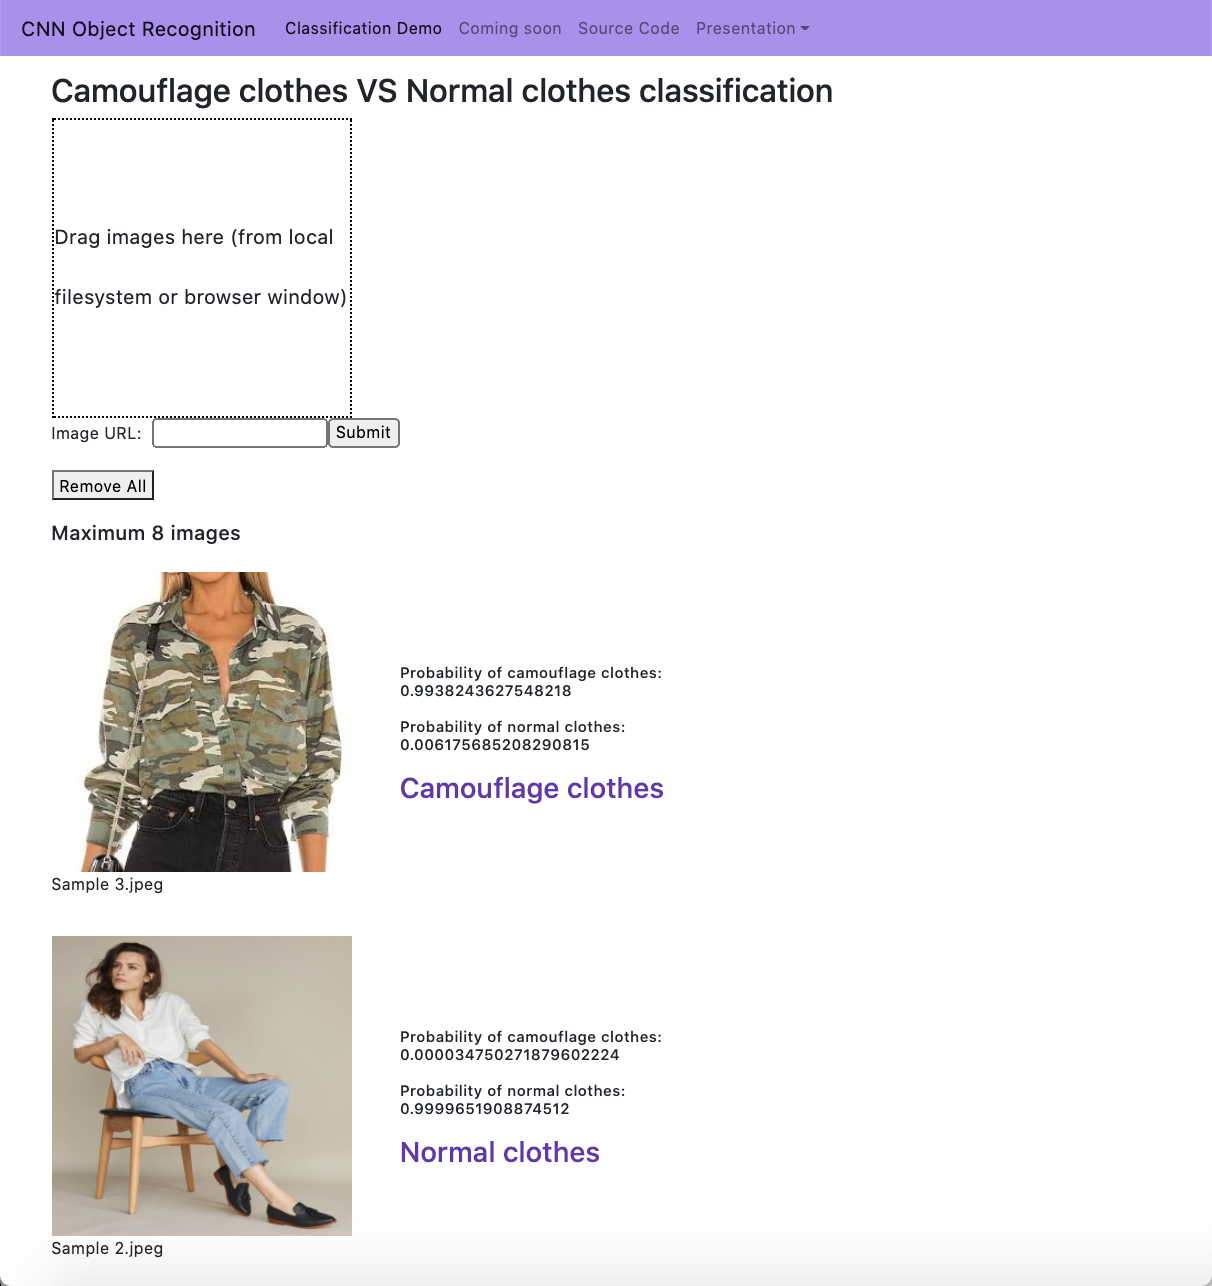
\includegraphics[width=0.5\columnwidth]{screenshot.png} % Example image
\end{center}

\section*{\large{2 \hspace{10pt} Concepts}}
Building a CNN model from scratch with random weight initialization has two major shortcomings [2]. First, large amount of data are required to collect and process to achieve high accuracy. Second, training from scratch is computationally expensive and memory-demanding. Fine-tuning, which is a type of transfer learning, can significantly reduce the number of training data and computational resources required. Data augmentation further lowers the barrier of preparing for a sufficiently large and representative dataset. Therefore, it is crucial to understand transfer learning, fine-tuning and data augmentation.

\subsection*{2.1 \hspace{10pt} Transfer Learning}
Transfer learning takes a network pre-trained on a dataset and transfers knowledge learnt from the previous training to the new task. Transfer learning is proven to help improve the accuracy and training time of CNNs [2, 3].
For startup companies and individual learners, it is too demanding to train their models from scratch. Therefore, they typically repurpose pre-trained models such as VGG19, ResNet50, Faster R-CNN and YOLO built by tech giants and star researchers to solve their specific tasks.

\subsection*{2.2 \hspace{10pt} Fine-tuning}
There are two approaches to transfer learning. They are feature extraction and fine-tuning.
Feature extraction in transfer learning is the process of using pre-trained network as a feature extractor to extract feature vectors and then feeding these feature vectors together with optional labels to a machine learning algorithm for training. Fine-tuning in transfer learning is the process of re-training the CNN in which at least some of the parameters are added or changed. It has been demonstrated that fine-tuning can boost the task accuracy when the dataset is small and different from the pre-trained model’s dataset [4]. Intuitively, since the dataset is small, it must rely on the pre-trained model to learn more basic geometric shapes. When the dataset is different from the pre-trained model's dataset, for example, knowing whether an object is a clothes is not directly helpful for differentiating clothes of different styles without adding more knowledge on top of the previous visual cognition.

\subsection*{2.3 \hspace{10pt} Data Augmentation}
Data augmentation is a process of applying random transformations, such as flipping, shifting, rotation, zooming, changing brightness and changing colours, to increase the diversity of training data to reduce overfitting. Indeed, the original batch is replaced by the new randomly transformed batch. As real-world data can have great variance in terms of transformation, training data need to capture them. Since it is difficult and expensive to obtain training data under a comprehensive set of transformations, data augmentation allows the training data to generalize better and easier.

\section*{\large{3 \hspace{10pt} Implementations}}

\subsection*{3.1 \hspace{10pt} Image Classification}
In this project, an image classification example is already developed and an object detection example will be developed. For image classification example, 99\% validation accuracy and 98\% testing accuracy are already achieved and prediction of each image is completed within 0.07 second using tensorflow model in python and a desktop with i7-10700 CPU and 32GB RAM. Using tensorflow model in javascript and the same desktop, prediction time is approximately doubled. Since image classification tasks are generally more analytical rather than about real-time monitoring, such latency and testing time are sufficient. It is believed that 98\% testing accuracy is likely sufficient for readers to persuade themselves, their bosses, their colleagues and even investors to kick-start their project, while keeping this example simple enough for readers to get started. Testing accuracy can be further improved by larger dataset, better hyper-parameter tuning and re-training more layers. \\
\\
ResNet50 is used as the base model for re-training. ResNet50 has higher accuracy than AlexNet, VGGNet and GoogLeNet. Besides, it is shown that ResNet is relatively easy to train, tolerant of hyper-parameters and generalizes well [5]. ResNet50 is chosen among ResNet variants since it is believed that ResNet50 strikes a good balance between accuracy and training time. Deeper ResNet architectures have higher accuracy but longer training time. For start-up companies and individual learners with limited computational resources, training time and time due to trial and error should be restricted. In fine-tuning, the last fully connected dense layer for prediction is first removed. Then, a pooling layer, flatten layer, dense layer of 256 neurons, dropout layer and dense layer of 2 neurons for prediction are added in order. Only these added layers are trained while layers from the base model are frozen. Pooling layer reduces computational cost and reduces overfitting. Flatten layer reshapes the tensor from the pooling layer. Dropout layer reduces inter-dependent learning among the neurons and thus reduces overfitting. The first dense layer takes previous knowledge and provides learning features. The second dense layer classifies the image and outputs class labels.

\subsection*{3.2 \hspace{10pt} Object Detection}
On the other hand, object detection tasks generally emphasize on latency and frames per second (FPS) to accomplish real-time monitoring. This example has not been implemented yet. The model is aimed to achieve 30 FPS and 10\% mean average precision (mAP) measured at 50\% intersection over union (IOU) using the same desktop with i7-10700 CPU and 32GB RAM [6]. Since it is expensive for startup companies and individual learners to set up high-end GPUs, it is difficult to achieve both high FPS and high mAP at the same time. It is believed that for a deployable solution, low mAP can still deal with typical cases well and can be compensated by other parts of the application, while a fairly good FPS should not be compromised. Otherwise, real-time user interactions and real-time control systems become infeasible as the whole pipeline is bottlenecked by this object detection task. It is hoped that readers succeed to develop real-time applications such as games and autonomous robot plugins. \\
\\
YOLOv3-tiny will be used as the base model for re-training. Although YOLO cannot localize some objects precisely and the number of nearby objects that YOLO can predict is restricted [7], YOLO is much faster than other state-of-the-art systems. For example, YOLO is three times faster than SSD [8]. Systems such as R-CNN, Fast R-CNN and Faster R-CNN generate region proposals and then classify the objects inside. Despite the fact that these systems allow more fine-grained object detection, they are especially not considered in real-time systems mainly because generating region proposals are very time-consuming. YOLO is proved to accomplish real-time performance when connected to a webcam by the research team [7], which is promising. YOLOv3-tiny is chosen among YOLO variants to ensure that the model is sufficiently lightweight and fast to re-train.

\section*{\large{4 \hspace{10pt} References}}
\noindent{[1] \href{https://ijcsit.com/docs/Volume\%207/vol7issue5/ijcsit20160705014.pdf}{https://ijcsit.com/docs/Volume\%207/vol7issue5/ijcsit20160705014.pdf}}

\noindent{[2] \href{https://openreview.net/pdf?id=ryxyCeHtPB}{https://openreview.net/pdf?id=ryxyCeHtPB}}

\noindent{[3] \href{https://www.researchgate.net/profile/Jordan-Bird/publication/
325803364\_A\_Study\_on\_CNN\_Transfer\_Learning\_for\_Image\_Classification/links/5bd8874b92851c6b279a23ea/A-Study-on-CNN-Transfer-Learning-for-Image-Classification.pdf}{https://www.researchgate.net/profile/Jordan-Bird/publication/
325803364\_A\_Study\_on\_CNN\_Transfer\_Learning\_for\_Image\_Classification/links/5bd8874b92851c6b279a23ea/A-Study-on-CNN-Transfer-Learning-for-Image-Classification.pdf}}

\noindent{[4] \href{https://arxiv.org/pdf/1406.2952.pdf}{https://arxiv.org/pdf/1406.2952.pdf}}

\noindent{[5] \href{https://arxiv.org/pdf/1603.05027.pdf}{https://arxiv.org/pdf/1603.05027.pdf}}

\noindent{[6] \href{https://arxiv.org/pdf/1907.11093.pdf}{https://arxiv.org/pdf/1907.11093.pdf}}

\noindent{[7] \href{https://openaccess.thecvf.com/content\_cvpr\_2016/papers/Redmon\_You\_Only\_Look\_CVPR\_2016\_paper.pdf}{https://openaccess.thecvf.com/content\_cvpr\_2016/papers/Redmon\_You\_Only\_Look\_CVPR\_2016\_paper.pdf}}

\noindent{[8] \href{https://arxiv.org/pdf/1804.02767.pdf}{https://arxiv.org/pdf/1804.02767.pdf}}

\end{document}